%
%===============>>  ГРУППА 11-2 МОДУЛЬ 8  <<=============
%
\setmodule{8}

%BEGIN_FOLD % ====>>_____ Занятие 1 _____<<====
\begin{class}[number=1]
	\begin{listofex}
		\item
		\begin{minipage}[t]{\bodywidth}
			На рисунке изображён график функции \[ f(x)=a \cos{x}+b \] Найдите \(a\).
		\end{minipage}
		\hspace{0.02\linewidth}
		\begin{minipage}[t]{\picwidth}
			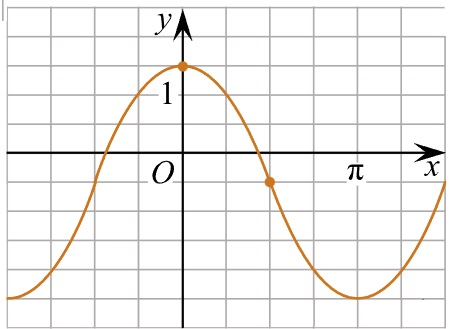
\includegraphics[align=t, width=\linewidth]{\picpath/MECGERM6H3-1}
		\end{minipage}
		%?
		\item
		\begin{minipage}[t]{\bodywidth}
			На рисунке изображён график функции \[ f(x)=a \tg{x}+b \] Найдите \(a\).
		\end{minipage}
		\hspace{0.02\linewidth}
		\begin{minipage}[t]{\picwidth}
			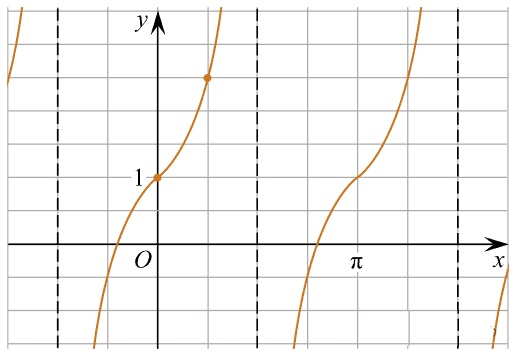
\includegraphics[align=t, width=\linewidth]{\picpath/MECGERM6H3-2}
		\end{minipage}
		\item %1 параболы
		\begin{minipage}[t]{\bodywidth}
			На рисунке изображены графики функций \(f(x) = 4x^2-25x+41 \) и \( g(x)=ax^2+bx+c \), которые пересекаются в точках \(A\) и \(B\). Найдите абсциссу точки \(B\).
		\end{minipage}
		\hspace{0.02\linewidth}
		\begin{minipage}[t]{\picwidth}
			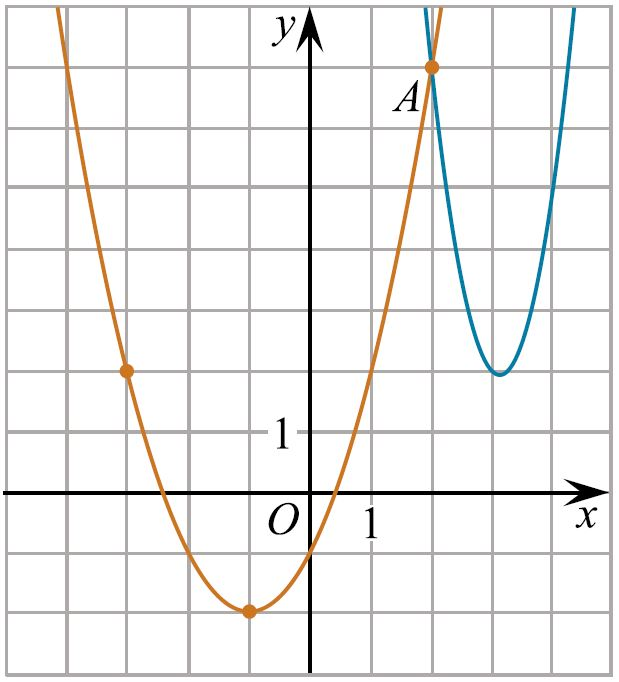
\includegraphics[align=t, width=\linewidth]{../pics/G112M3C1-10}
		\end{minipage}
		\item %1 LOGARIFM
		\begin{minipage}[t]{\bodywidth}
			На рисунке изображен график функции \(f(x) = b+\log_ax \). Найдите \(f(32)\).
		\end{minipage}
		\hspace{0.02\linewidth}
		\begin{minipage}[t]{\picwidth}
			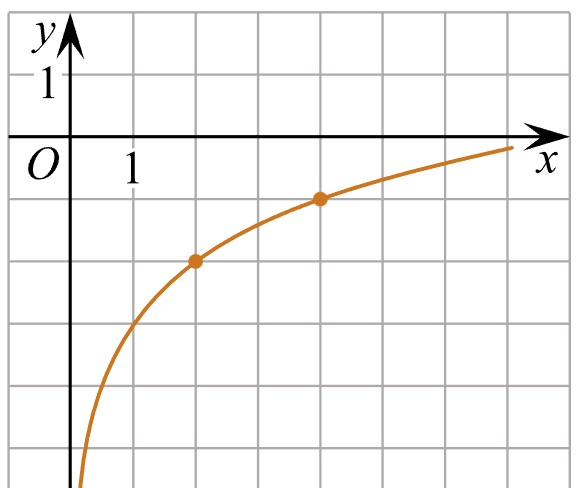
\includegraphics[align=t, width=\linewidth]{../pics/G111M8L1-1}
		\end{minipage}
		%\item %1 s golovi
		%\begin{minipage}[t]{\bodywidth}
		%	На рисунке изображен график функции \(f(x) = \dfrac{ x^2 }{ a }+bx+c \), где числа \(a, b, c\) --- целые. Найдите значение \(f(3,5)\).
		%\end{minipage}
		%\hspace{0.02\linewidth}
		%\begin{minipage}[t]{\picwidth}
		%	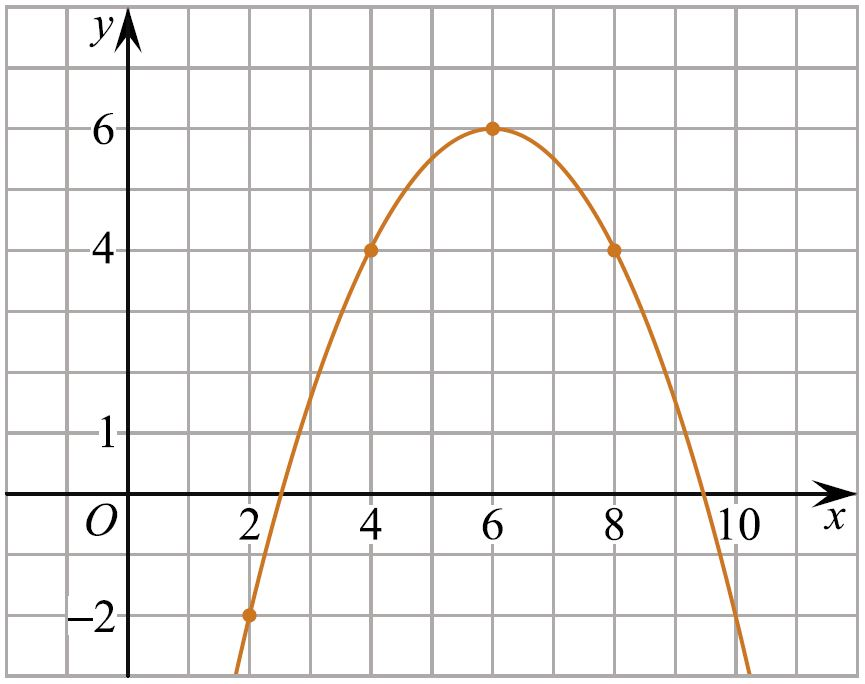
\includegraphics[align=t, width=\linewidth]{../pics/G112M3C1-6}
		%\end{minipage}
		\item Решите неравенства: %c193 23 24 27 28 a
		\begin{tasks}(2)
			\task \( \sqrt[4]{x^2-24x} \le 3 \)
			\task \( \sqrt[28]{8x-x^2-15} < 1 \)
			\task \( \sqrt[]{x^2-2x-15} < 3 \)
			\task \( \sqrt[]{3x^2-14x+51} \ge 6 \)
		\end{tasks}
		\item Решите неравенства:
		\begin{tasks}(1)
			\task \( \sqrt[]{x^4-2x+6} \ge x \)
			\task \( \sqrt[]{5x^4-28x^2+16} \ge x^2+4 \)
		\end{tasks}
		\newpage
		\item Решите неравенства: %с289 1 2 3 5 6 8
		\begin{tasks}(2)
			\task \( 4^{\tfrac{5}{x}} \ge 64 \)
			\task \( \left( \dfrac{ 1 }{ 3 } \right)^{\tfrac{ 3x+2 }{ 1-x }} < 81 \)
			
			\task \( 3^x \cdot \left( \dfrac{ 1 }{ 81 } \right)^{2x+3} < 9 \)
			\task \( 4^{3x-2}+4^{3x-1} \le 80 \)
			\task \( 5^{x-3}+5^{x-2}+5^{x-1} \ge 155 \)
			\task \( (0,2)^{\tfrac{x^2+11x+49}{2x-9}} \ge 5 \)
		\end{tasks}
	\end{listofex}
\end{class}
%END_FOLD

%BEGIN_FOLD % ====>>_____ Занятие 2 _____<<====
\begin{class}[number=2]
	\begin{listofex}
		\item Решить неравенство: 
		\[ 5^x+\dfrac{125}{5^x-126}\ge 0. \]
		\item Решить неравенство:
		\[ \dfrac{2}{5^x+75} \ge \dfrac{1}{5^x-25} \]
		\item Решить неравенство:
		\[ 16^{\tfrac{1}{x}-1}-4^{\tfrac{1}{x}-1}-2 \ge 0 \]
		\item Решить неравенство:
		\[ \dfrac{1}{2^x-1}+\dfrac{4^{x+\tfrac{1}{2}}-2^{x+5}+4}{2^x-16} \ge 2^{x+1} \]
		\item Решить неравенство:
		\[ 27\cdot45^x-27^{x+1}-12\cdot15^x+12\cdot9^x+5^x-3^x \le 0  \]
		\item Решить неравенство:
		\[ 2^{x+1}+\dfrac{9}{x}-\dfrac{3\cdot2^x}{x}\ge 6 \]
		\item Решить неравенство:
		\[ \dfrac{9^x+2 \cdot 3^x-117}{3^x-27} \le 1 \]
		\item Решить неравенство: \[ \dfrac{ 3^{|x^2-2x-1|}-9}{ x } \ge 0 \]
		
		
		\item Решить неравенство: \[ 64^{x^2-3x+20}-0,125^{2x^2-6x-200} \le 0 \]
		\item Решить неравенство: \[ 4^{x^2+x-3}-0,5^{2x^2-6x-2} \le 0 \]
	\end{listofex}
\end{class}
%END_FOLD

%BEGIN_FOLD % ====>>_ Домашняя работа 1 _<<====
\begin{homework}[number=1]
	\begin{listofex}
		\item Решите неравенства: %c192 n 25 26 27 28 b /c289 1 2 4 5 b
		\begin{tasks}(2)
			%\task \( \sqrt[3]{9x-x^2} \le 2 \)
			%\task \( \sqrt[]{x^2-25} \le 12 \)
			%\task \( \sqrt[]{x^2-4x-5} < 4 \)
			%\task \( \sqrt{4x^2-29x+61} \ge 3 \)
			%\task \( 3^{\tfrac{ 4 }{ x }} \ge 27 \)
			%\task \( 0,5^{\tfrac{ 3x-2 }{ 3-x }}<16 \)
			%\task \( \left( \dfrac{ 1 }{ 3 } \right)^{\tfrac{ 4x-1 }{ x-5 }} > 81^{\tfrac{ x-2 }{ x+5 }} \)
			%\task \( 6^x \cdot \left( \dfrac{ 1 }{ 36 } \right)^{5x+3} < 6 \)
			\task \( \dfrac{ 9^x-3^x-90 }{ 3^x-82 } \le 1 \)
			\task \( 2^{2x-1}-7 \cdot 2^{x-1}+5 \le 0 \)
			\task \( 2^x+80 \cdot 2^{4-x} \le 261 \)
			\task \( 2^{2x+4}-16 \cdot 2^{x+3}-2^{x+1}+16 \le 0 \)
			\task \( 6^x-4 \cdot 3^x-2^x+4 \le 0 \)
			\task \( 4^{x^2+x-3}-0,5^{2x^2-6x-2} \le 0 \)
		\end{tasks}
		%trigon10 8
		%\item
		%\begin{minipage}[t]{\bodywidth}
		%	На рисунке изображён график функции вида \[ f(x)= a\cos \left( \dfrac{ \pi x }{ b }+c \right)+d, \] где \(a,b,c, d\) --- целые. Найдите \(f\left( -\dfrac{ 22 }{ 3 } \right)\).
		%\end{minipage}
		%\hspace{0.02\linewidth}
		%\begin{minipage}[t]{\picwidth}
		%	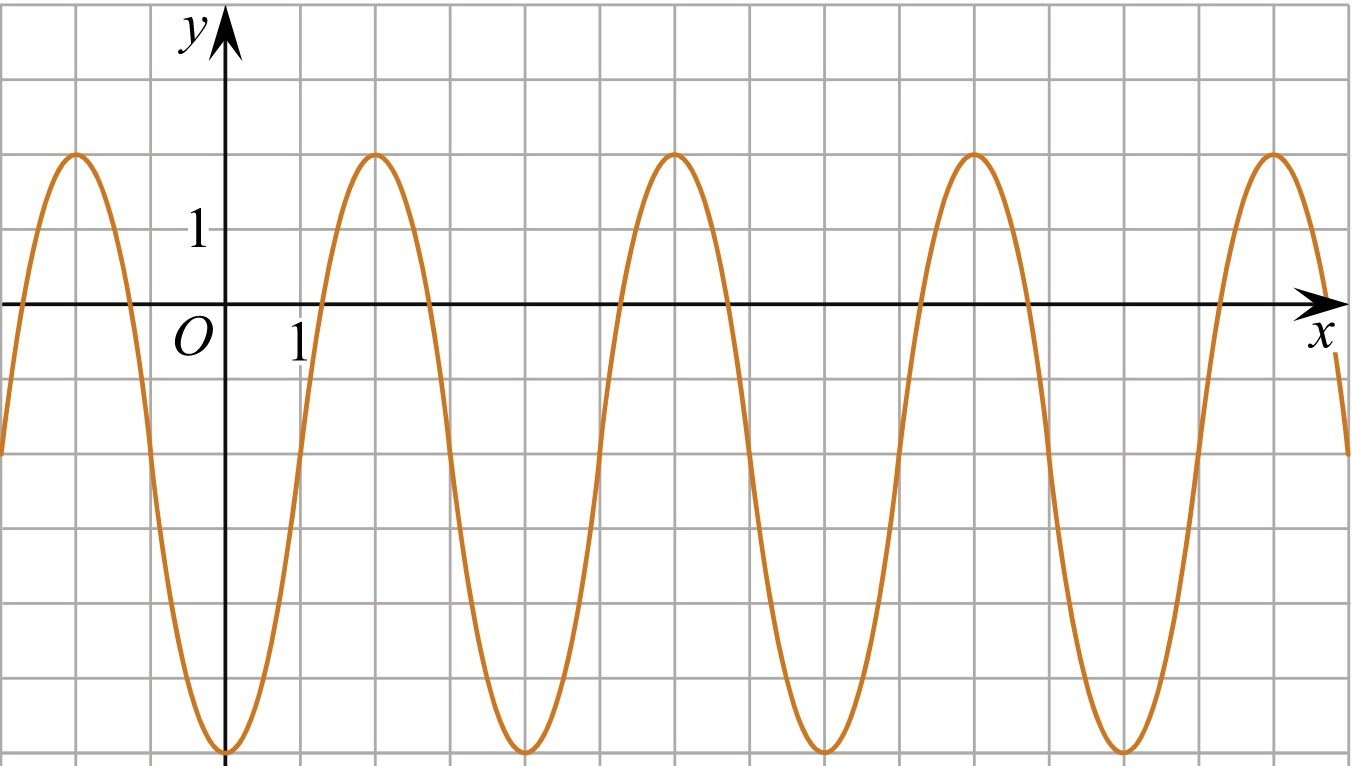
\includegraphics[align=t, width=\linewidth]{\picpath/G112M8H1-1}
		%\end{minipage}
	\end{listofex}
\end{homework}
%END_FOLD

%BEGIN_FOLD % ====>>_____ Занятие 3 _____<<====
\begin{class}[number=3]
	\begin{listofex}
		%11.1v2v3 po 3
		\item Найдите точку максимума функции \( y=x^3-48x+17 \).
		\item Найдите наименьшее значение функции \( y=x^3-27 \) на отрезке \([0;4]\).
		\item Найдите наибольшее значение функции \( y=x^3-3x+4 \) на отрезке \([-2;0]\).
		%1-4 analog 282861
		\item Найдите наименьшее значение функции \( y=(x+3)^2(x+5)-1 \) на отрезке \([-4;-1]\).
		\item Найдите наименьшее значение функции \( y=(x-7)^2(x+6) \) на отрезке \([-1;20]\).
		\item Найдите наименьшее значение функции \( y=(x-8)^2(x-1)+10 \) на отрезке \([6;14]\).
		\item Найдите наибольшее значение функции \( y=(x-2)^2(x-4)+5 \) на отрезке \([1;3]\).
		\item Найдите точку максимума функции \( y=-\dfrac{ x^2+289 }{ x } \).
		%\item Найдите точку минимума функции \( y=-\dfrac{ x^2+1 }{ x } \).
		\item Найдите наименьшее значение функции \( y=\dfrac{x^2+25  }{ x } \) на отрезке \([1;10]\).
		\item Найдите наименьшее значение функции \( y=(x-8)e^{x-7} \) на отрезке \([6;8]\).
		\item Найдите точку минимума функции \( y=(x+16)e^{x-16} \).
		\item Найдите точку максимума функции \( y=(9-x)e^{x+9} \).
		
		
		%G111M5L2
		%\item
		%\begin{minipage}[t]{\bodywidth}
		%	На рисунке изображен график функции \( y = f(x)\), определенной на интервале \((-5; 5)\). Найдите количество точек, в которых касательная к графику функции параллельна прямой \(y  =  6\) или совпадает с ней.
		%\end{minipage}
		%\hspace{0.02\linewidth}
		%\begin{minipage}[t]{\picwidth}
		%	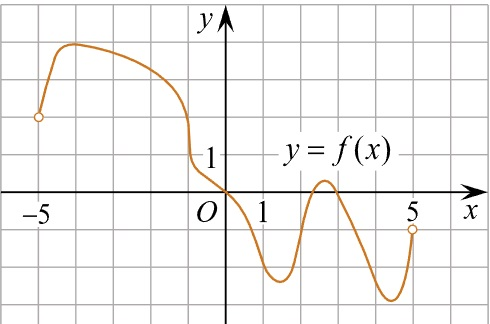
\includegraphics[align=t, width=\linewidth]{\picpath/G111M5L2-1}
		%\end{minipage}
		%\item
		%\begin{minipage}[t]{\bodywidth}
		%	На рисунке изображен график производной функции \(f(x)\), определенной на интервале \((-10; 2)\). Найдите количество точек, в которых касательная к графику функции \(f(x)\) параллельна прямой \(y = -2x - 11\) или совпадает с ней.
		%\end{minipage}
		%\hspace{0.02\linewidth}
		%\begin{minipage}[t]{\picwidth}
		%	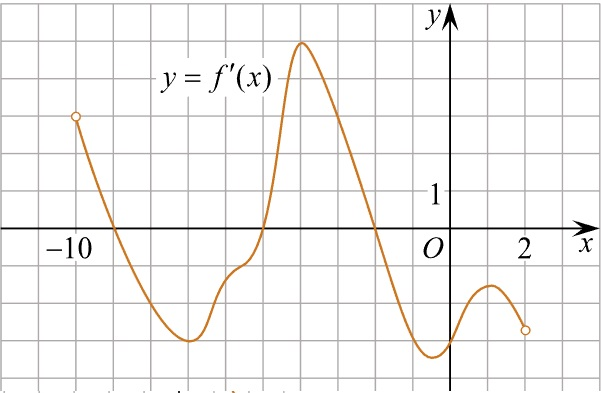
\includegraphics[align=t, width=\linewidth]{\picpath/G111M5L2-2}
		%\end{minipage}
		%G111M5L2
		\item
		\begin{minipage}[t]{\bodywidth}
			На рисунке изображен график производной функции \(f(x)\) , определенной на интервале \( (-6;6) \) . Найдите промежутки возрастания функции \(f(x)\) . В ответе укажите сумму целых точек, входящих в эти промежутки.
		\end{minipage}
		\hspace{0.02\linewidth}
		\begin{minipage}[t]{\picwidth}
			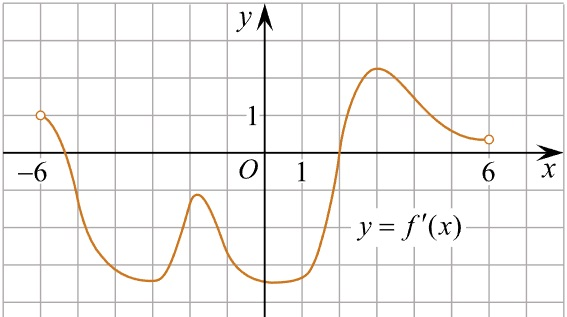
\includegraphics[align=t, width=\linewidth]{\picpath/G111M5L2-3}
		\end{minipage}
		\item
		\begin{minipage}[t]{\bodywidth}
			На рисунке изображен график функции \(y = f(x)\), определенной на интервале \((-6; 8)\). Определите количество целых точек, в которых производная функции положительна.
		\end{minipage}
		\hspace{0.02\linewidth}
		\begin{minipage}[t]{\picwidth}
			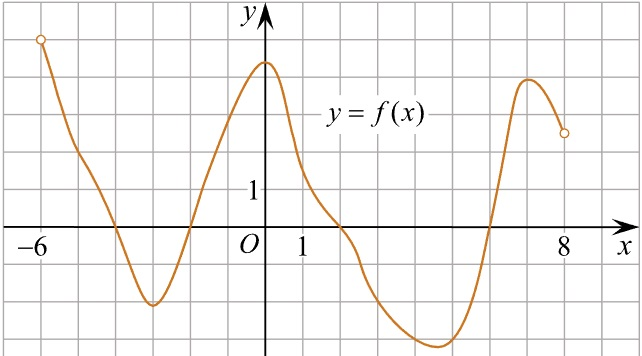
\includegraphics[align=t, width=\linewidth]{\picpath/G111M5L2-4}
		\end{minipage}
		%525690
		\item
		\begin{minipage}[t]{\bodywidth}
			На рисунке изображены график функции \(y=f(x)\) и касательная к этому графику, проведённая в точке \(x_0\). Уравнение касательной показано на рисунке. Найдите значение производной функции \(g(x)=-7f(x)+21x+\dfrac{ 1 }{ 441 }\) в точке \(x_0\).
		\end{minipage}
		\hspace{0.02\linewidth}
		\begin{minipage}[t]{\picwidth}
			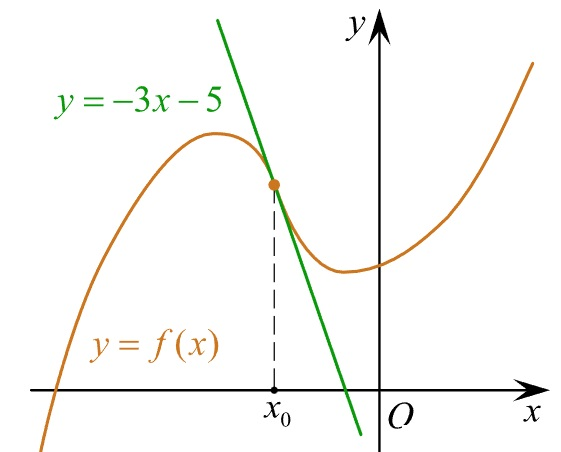
\includegraphics[align=t, width=\linewidth]{\picpath/G112M8C3-1}
		\end{minipage}
		%525702
		\item
		\begin{minipage}[t]{\bodywidth}
			На рисунке изображены график функции \(y=f(x)\) и касательная к этому графику, проведённая в точке \(x_0\). Уравнение касательной показано на рисунке. Найдите значение производной функции \(g(x)=-5f(x)-\dfrac{ 2 }{ 11 }x+\ln3\) в точке \(x_0\).
		\end{minipage}
		\hspace{0.02\linewidth}
		\begin{minipage}[t]{\picwidth}
			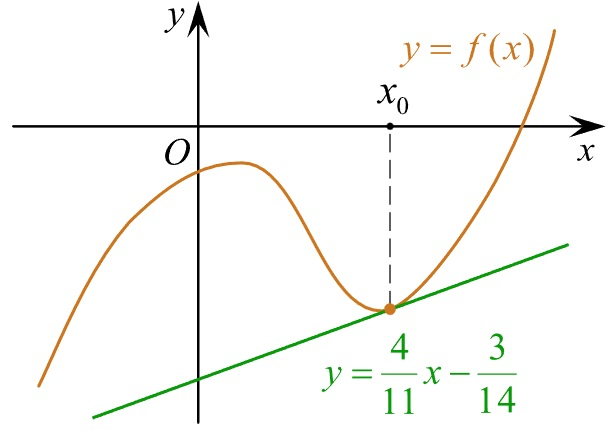
\includegraphics[align=t, width=\linewidth]{\picpath/G112M8C3-2}
		\end{minipage}
		%525691
		\item
		\begin{minipage}[t]{\bodywidth}
			На рисунке изображены график функции \(y=f(x)\) и касательная к этому графику, проведённая в точке \(x_0\). Уравнение касательной показано на рисунке. Найдите значение производной функции \(g(x)=(f'(x)-0,5)\cdot 6\) в точке \(x_0\).
		\end{minipage}
		\hspace{0.02\linewidth}
		\begin{minipage}[t]{\picwidth}
			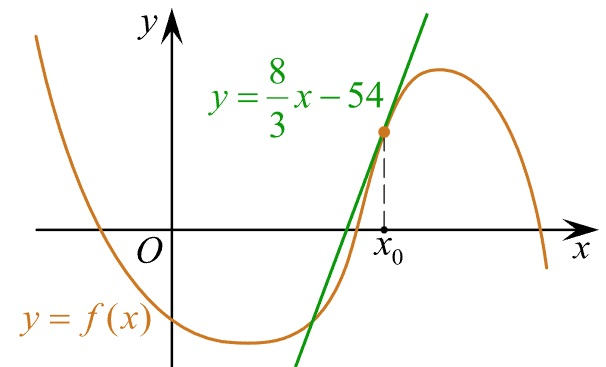
\includegraphics[align=t, width=\linewidth]{\picpath/G112M8C3-3}
		\end{minipage}
		%525703
		\item
		\begin{minipage}[t]{\bodywidth}
			На рисунке изображены график функции \(y=f(x)\) и касательная к этому графику, проведённая в точке \(x_0\). Уравнение касательной показано на рисунке. Найдите значение производной функции \(g(x)=f'(x)-f(x)+3\) в точке \(x_0\).
		\end{minipage}
		\hspace{0.02\linewidth}
		\begin{minipage}[t]{\picwidth}
			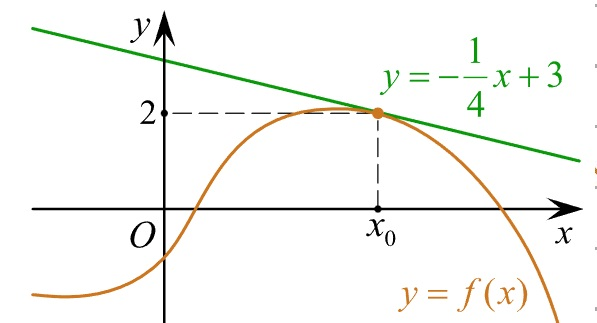
\includegraphics[align=t, width=\linewidth]{\picpath/G112M8C3-4}
		\end{minipage}
		\item
		\begin{minipage}[t]{\bodywidth}
			На рисунке изображены графики функций \(f(x)=5x+9\) и \( g(x)=ax^2+bx+c \), которые пересекаются в точках \(A\) и \(B\). Найдите абсциссу точки \(B\).
		\end{minipage}
		\hspace{0.02\linewidth}
		\begin{minipage}[t]{\picwidth}
			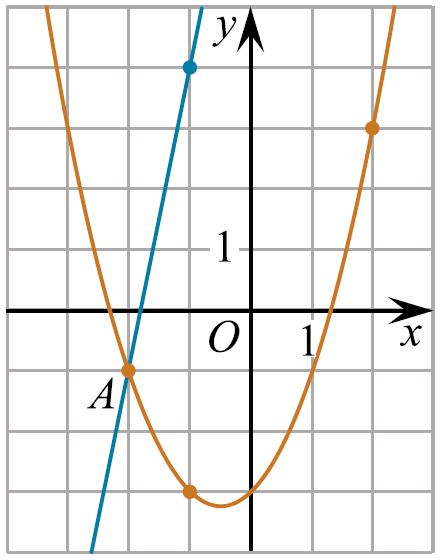
\includegraphics[align=t, width=\linewidth]{\picpath/G112M3C1-9}
		\end{minipage}
		
		\item
		\begin{minipage}[t]{\bodywidth}
			На рисунке изображен график функции \( f(x)=\dfrac{k}{x}+a \). Найдите, при каком значении \( x \) значение функции будет равно \( 0,8 \).
		\end{minipage}
		\hspace{0.02\linewidth}
		\begin{minipage}[t]{\picwidth}
			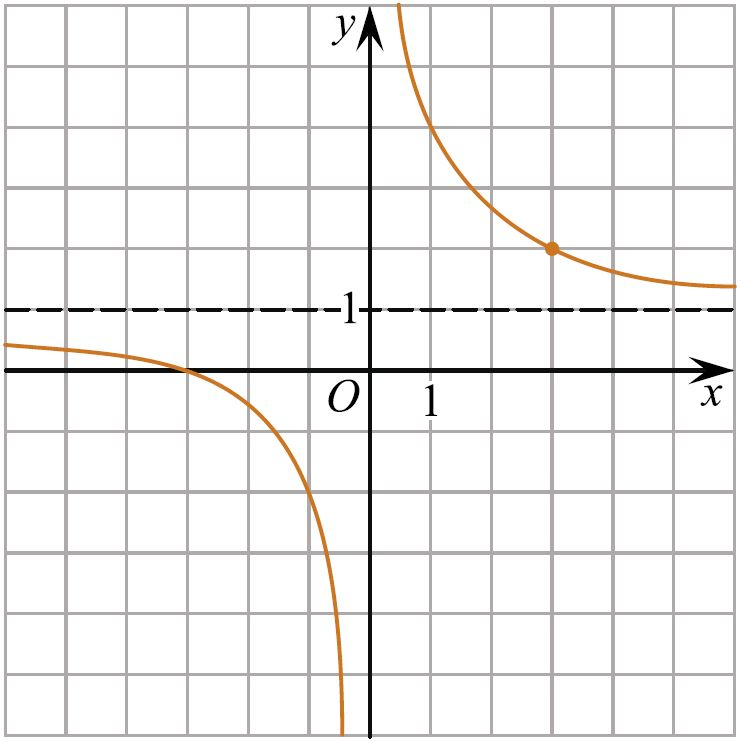
\includegraphics[align=t, width=\linewidth]{\picpath/G112M3C2-5}
		\end{minipage}
		\item %1 LOGARIFM
		\begin{minipage}[t]{\bodywidth}
			На рисунке изображен график функции \(f(x) = b+\log_ax \). Найдите \(f(32)\).
		\end{minipage}
		\hspace{0.02\linewidth}
		\begin{minipage}[t]{\picwidth}
			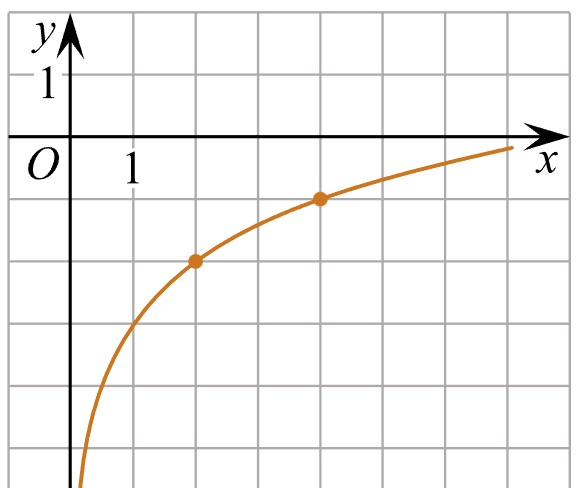
\includegraphics[align=t, width=\linewidth]{../pics/G111M8L1-1}
		\end{minipage}
	\end{listofex}
\end{class}
%END_FOLD

%BEGIN_FOLD % ====>>_____ Занятие 4 _____<<====
\begin{class}[number=4]
	\begin{listofex}
		\item Решите неравенства: %c298 a 1 2 4 6 7 8 9 10
		\begin{tasks}(2)
			\task \( \log_x<2 \)
			\task \( \log_3x\le3 \)
			\task \( \log_{0,123}x \le 0 \)
			\task \( \log_{0,04}x \ge -1 \)
			\task \( \log_5 (4x+5) < 3 \)
			\task \( \log_{0,1}(3x+25)<-2 \)
			\task \( \log_{\tfrac{2}{7}}(2x-2,5)\le -1 \)
			\task \( \log_3 (10x-19)>4 \)
		\end{tasks}
	\end{listofex}
\end{class}
%END_FOLD

%BEGIN_FOLD % ====>>_ Домашняя работа 2 _<<====
\begin{homework}[number=2]
	\begin{listofex}
		%11.1v2v3 po 4-5
		%\item Найдите наибольшее значение функции \(y=\sqrt{5-4x-x^2}\).
		\item 
		\begin{tasks}
			\task Решите уравнение: \( \cos 2x = \sin \left( x+\dfrac{ \pi }{ 2 } \right) \)
			\task Найдите корни этого уравнения, принадлежащие промежутку \( [-2\pi; -\pi] \).
		\end{tasks}
		\item Решите неравенство: \( \log^2_2 x + 6 > 5\log_2 x \).
		
		\item Решите неравенство: \( \dfrac{ 9^x-3^x-90 }{3^x-82  } \le 1 \).
		\item Решите неравенство: \(\log_{125}(2x^2+x-3) \ge \dfrac{ 2 }{ 3 }\).
		
		\item Решите неравенство: \( \dfrac{ 5\lg^2x-1 }{ \lg^2x -1}\ge1 \).
		\item Решите неравенство: \( \dfrac{ 1 }{ 4+\log_2x }+\dfrac{ 2 }{ \log_2(2x) }\left( \dfrac{ 3 }{ 4+\log_2x }-1 \right) \le 1 \).
		\item Решите неравенство: \( \dfrac{ \log_4(2^x-2)}{ x-1,5 } \le 1 \).
		\item Решите неравенство: \( \log_{x+1}(6x^2+x-5)<2 \).
		\item Найдите точку максимума функции \(y=\log_2 (2+2x-x^2)-2\).
		
		\item Найдите точку максимума функции \(y=x^3-3x^2+2\).
		\item Найдите точку минимума функции \(y=x^3-5x^2-14\).
		
		\item Найдите наибольшее значение функции \(y=\dfrac{ x^2+25 }{ x }\) на отрезке \(\left[ -10;-1 \right]\).
		\item Найдите точку максимума функции \(y=\dfrac{ 16 }{ x }+x+3\).
		
		
		\item Материальная точка движется прямолинейно по закону \( x(t)=6t^2-48t+17 \) (где \(x\) --- расстояние от точки отсчета в метрах, \(t\) --- время в секундах, измеренное с начала движения). Найдите ее скорость (в м/с) в момент времени \(t  =  9\) с.
		%
		\item
		\begin{minipage}[t]{0.5\linewidth}
			На рисунке изображен график функции \(y = f(x)\), определенной на интервале \((-6; 5)\). Найдите количество точек, в которых касательная к графику функции параллельна прямой \(y=-6\).
		\end{minipage}
		\hspace{0.02\linewidth}
		\begin{minipage}[t]{0.45\linewidth}
			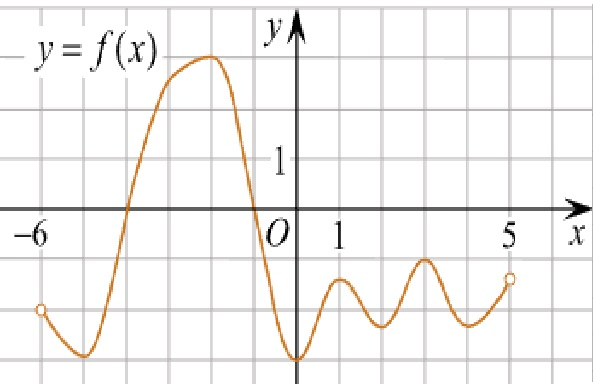
\includegraphics[align=t, width=\linewidth]{../pics/G111M3H2-4}
		\end{minipage}
		
	\end{listofex}
\end{homework}
%END_FOLD

%BEGIN_FOLD % ====>>_____ Занятие 5 _____<<====
\begin{class}[number=5]
	\begin{listofex}
		%N9 1V2V3 по 2 первые
		\item В \(2008\) году в городском квартале проживало \(40 000\) человек. В \(2009 \) году, в результате строительства новых домов, число жителей выросло на \(8 \%\), а в \(2010\) году на \(9 \%\) по сравнению с \(2009\) годом. Сколько человек стало проживать в квартале в \(2010\) году?
		\item В понедельник акции компании подорожали на некоторое количество процентов, а во вторник подешевели на то же самое количество процентов. В результате они стали стоить на \(4 \%\) дешевле, чем при открытии торгов в понедельник. На сколько процентов подорожали акции компании в понедельник?
		
		
		\item Из пункта \(A\) в пункт \(B\) одновременно выехали два автомобиля. Первый проехал с постоянной скоростью весь путь. Второй проехал первую половину пути со скоростью, меньшей скорости первого на \(13\) км/ч, а вторую половину пути --- со скоростью \(78\) км/ч, в результате чего прибыл в пункт \(B\) одновременно с первым автомобилем. Найдите скорость первого автомобиля, если известно, что она больше \(48\) км/ч. Ответ дайте в км/ч.
		
		\item Два мотоциклиста стартуют одновременно в одном направлении из двух диаметрально противоположных точек круговой трассы, длина которой равна \(14\) км. Через сколько минут мотоциклисты поравняются в первый раз, если скорость одного из них на \(21\) км/ч больше скорости другого?
		\item Из одной точки круговой трассы, длина которой равна \(14\) км, одновременно в одном направлении стартовали два автомобиля. Скорость первого автомобиля равна \(80\) км/ч, и через \(40\) минут после старта он опережал второй автомобиль на один круг. Найдите скорость второго автомобиля. Ответ дайте в км/ч.
		
		%voda 1 4
		\item Моторная лодка прошла против течения реки \(112\) км и вернулась в пункт отправления, затратив на обратный путь на \(6\) часов меньше. Найдите скорость течения, если скорость лодки в неподвижной воде равна \(11\) км/ч. Ответ дайте в км/ч.
		\item Теплоход проходит по течению реки до пункта назначения \(200\) км и после стоянки возвращается в пункт отправления. Найдите скорость течения, если скорость теплохода в неподвижной воде равна \(15\) км/ч, стоянка длится \(10\) часов, а в пункт отправления теплоход возвращается через \(40\) часов после отплытия из него. Ответ дайте в км/ч.
		
		%analogi splav 7 и 8 первые
		\item Смешали некоторое количество \(13\)-процентного раствора некоторого вещества с таким же количеством \(17\)-процентного раствора этого вещества. Сколько процентов составляет концентрация получившегося раствора?
		\item В сосуд, содержащий \(7\) литров \(14\)-процентного водного раствора некоторого вещества, добавили \(7\) литров воды. Сколько процентов составляет концентрация получившегося раствора?
		%splav10
		\item Изюм получается в процессе сушки винограда. Сколько килограммов винограда потребуется для получения \(20\) килограммов изюма, если виноград содержит \(90\%\) воды, а изюм содержит \(5\%\) воды?
		
		%sovmest rabota 10, 11, 17
		\item Один мастер может выполнить заказ за \(12\) часов, а другой --- за \(6\) часов. За сколько часов выполнят заказ оба мастера, работая вместе?
		\item Первый садовый насос перекачивает \(5\) литров воды за \(2\) минуты, второй насос перекачивает тот же объём воды за \(3\) минуты. Сколько минут эти два насоса должны работать совместно, чтобы перекачать \(25\) литров воды?
		\item Каждый из двух рабочих одинаковой квалификации может выполнить заказ за \(15\) часов. Через \(3\) часа после того, как один из них приступил к выполнению заказа, к нему присоединился второй рабочий, и работу над заказом они довели до конца уже вместе. Сколько часов потребовалось на выполнение всего заказа?
		
		%analogi 77382 1-4
		\item Решите уравнения, если уравнение имеет более одного корня, в ответе запишите меньший из корней:
		\begin{tasks}(2)
			\task \( \log_{x-2}16=2 \)
			\task \( \log_{x-1}81=2 \)
			\task \( \log_{x-7}25=2 \)
			\task \( \log_{x-3}16=2 \)
		\end{tasks}
		%14log 1 2 3
		%\item Решите неравенство: \( \log_3 \dfrac{ 1 }{ x }+\log_3(x^2+3x-9) \le \log_3 (x^2+3x+\dfrac{ 1 }{ x }-10) \)
		%\item Решите неравенство: \( 9\log_7(x^2+x-2)\le 10 + \log_7 \dfrac{ (x-1)^9 }{ x+2 } \)
		%\item Решите неравенство: \( \log_2 (x^2-4)-3\log_2 \dfrac{ x+2 }{ x-2 } > 2 \)
		
		\item Решите неравентсва: %c299 n30 31 34 a
		\begin{tasks}
			\task \( \log_9(2x^2+7x+5)\ge 1,5 \)
			\task \( \log_{64}(5x^2-4x-12) \le \dfrac{ 2 }{ 3 } \)
			\task \( \log_2(5x+7) < \log_2 (3x+11) \)
		\end{tasks}
	\end{listofex}
\end{class}
%END_FOLD

%BEGIN_FOLD % ====>>_____ Занятие 6 _____<<====
\begin{class}[number=6]
	\begin{listofex}
		\item Из пункта \(A\) в пункт \(B\) одновременно выехали два автомобиля. Первый проехал с постоянной скоростью весь путь. Второй проехал первую половину пути со скоростью \(24\) км/ч, а вторую половину пути --- со скоростью, на \(16\) км/ч большей скорости первого, в результате чего прибыл в пункт \(B\) одновременно с первым автомобилем. Найдите скорость первого автомобиля. Ответ дайте в км/ч.
	\end{listofex}
\end{class}
%END_FOLD

%BEGIN_FOLD % ====>>_ Домашняя работа 3 _<<====
\begin{homework}[number=3]
	\begin{listofex}
		\item Домашняя работа 3
	\end{listofex}
\end{homework}
%END_FOLD

%BEGIN_FOLD % ====>>_____ Занятие 7 _____<<====
\begin{class}[number=7]
	\begin{listofex}
		%Всего по 3 первых
		\item В треугольнике \(ABC\): \(\angle C=90\degree \), \(AC\) --- один из катетов и равен \(4,8\), \(\sin A = \dfrac{ 7 }{ 25 }\). Найдите \(AB\).
		\item В треугольнике \(ABC\): \( \angle C =90\degree\), \(AC  = 4\), \(\cos A = 0,5\). Найдите \(AB\).
		\item В треугольнике \(ABC\): \(AC=BC=5\), \(\sin A = \dfrac{ 7 }{ 25 }\). Найдите \(AB\).
		\item В треугольнике \(ABC\): \(AC=BC, AB=9,6\), \(\cos A = \dfrac{ \sqrt{2} }{ 2 }\). Найдите \(AC\).
		\item Площадь треугольника \(ABC\) равна \(4\), \(DE\) --- средняя линия, параллельная стороне \(AB\). Найдите площадь треугольника \(CDE\).
		\item В параллелограмме \(ABCD: AB=3, AD=21, \sin A = \dfrac{ 6 }{ 7 }\). Найдите большую высоту параллелограмма.
		\item Найдите площадь квадрата, если его диагональ равна \(1\).
		\item Площадь прямоугольника равна \(18\). Найдите его большую сторону, если она на 3 больше меньшей стороны.
		\item Основания равнобедренной трапеции равны \(51\) и \(65\). Боковые стороны равны \(25\). Найдите синус острого угла трапеции.
		\item Основания равнобедренной трапеции равны \(43\) и \(73\). Косинус острого угла трапеции равен: \(\dfrac{ 5 }{ 7 }\).  Найдите боковую сторону.
		%\item Основания равнобедренной трапеции равны \(7\) и \(51\). Тангенс острого угла равен \(\dfrac{ 5 }{ 11 }\). Найдите высоту трапеции.
		\item Средняя линия трапеции равна \(28\), а меньшее основание равно \(18\). Найдите большее основание трапеции.
		\item Треугольник \(ABC\) вписан в окружность с центром \(O\). Найдите угол \(BOC\), если угол \(BAC\) равен \(32 \degree \).
		\item Найдите центральный угол \(AOB\), если он на \(15 \degree\) больше вписанного угла \(ACB\), опирающегося на ту же дугу. Ответ дайте в градусах.
		\item Найдите хорду, на которую опирается угол \(30\degree\), вписанный в окружность радиуса \(3\).
		\item Найдите хорду, на которую опирается угол \(120\degree \), вписанный в окружность радиуса \(\sqrt{3}\).
		\item Радиус вписанной в квадрат окружности равен \(3 \sqrt{2}\). Найдите радиус окружности, описанной около этого квадрата.
		\item Имеется два сплава. Первый сплав содержит \(10\%\) меди, второй --- \(40\%\) меди. Масса второго сплава больше массы первого на \(3\) кг. Из этих двух сплавов получили третий сплав, содержащий \(30\%\) меди. Найдите массу третьего сплава. Ответ дайте в килограммах.
		\item Имеется два сплава. Первый содержит \(10\%\) никеля, второй --- \(30\%\) никеля. Из этих двух сплавов получили третий сплав массой \(200\) кг, содержащий \(25\%\) никеля. На сколько килограммов масса первого сплава была меньше массы второго?
		\item Имеются два сосуда. Первый содержит \(30\) кг, а второй --- \(20\) кг раствора кислоты различной концентрации. Если эти растворы смешать, то получится раствор, содержащий \(68\%\) кислоты. Если же смешать равные массы этих растворов, то получится раствор, содержащий \(70\%\) кислоты. Сколько килограммов кислоты содержится в первом сосуде?
		
	\end{listofex}
\end{class}
%END_FOLD

%BEGIN_FOLD % ====>>_ Проверочная работа _<<====
\begin{exam}
	\begin{listofex}
		\item Проверочная
	\end{listofex}
\end{exam}
%END_FOLD

%\item Решите неравенства: %192 25 27 28 a
%\begin{tasks}(2)
%	\task \( \sqrt[3]{6x-x^2} \le 2 \)
%	\task \( \sqrt[]{x^2-2x-15}<3 \)
%	\task \( \sqrt[]{3x^2-14x+51} \ge 6 \)
%	\task \( \sqrt[]{x^2-144} \le 5 \)
%	\task \( \sqrt[]{x^4-2x+6} \ge x \)
%	\task \( \sqrt[]{5x^4-28x^2+16} \ge x^2+4 \)
%\end{tasks}
%\item Решите неравенства: %с289 1 2 3 5 6 8
%\begin{tasks}(2)
%	\task \( 4^{\tfrac{5}{x}} \ge 64 \)
%	\task \( \left( \dfrac{ 1 }{ 3 } \right)^{\tfrac{ 3x+2 }{ 1-x }} < 81 \)
%	
%	\task \( 3^x \cdot \left( \dfrac{ 1 }{ 81 } \right)^{2x+3} < 9 \)
%	\task \( 4^{3x-2}+4^{3x-1} \le 80 \)
%	\task \( 5^{x-3}+5^{x-2}+5^{x-1} \ge 155 \)
%	\task \( (0,2)^{\tfrac{x^2+11x+49}{2x-9}} \ge 5 \)
%\end{tasks}

%BEGIN_FOLD % ====>>_ Консультация Борисов _<<====
\begin{consultation}
	\begin{listofex}
		\item Найдите площадь треугольника, две стороны которого равны \(8\) и \(12\), а угол между ними равен \(30 \degree\).
		\item Большее основание равнобедренной трапеции равно \(34\). Боковая сторона равна \(14\). Синус острого угла равен \( \dfrac{ 2\sqrt{10}}{ 7 } \). Найдите меньшее основание.
		%\item Основания равнобедренной трапеции равны \(7\) и \(51\). Тангенс острого угла равен \( \dfrac{ 5 }{ 11 } \).  Найдите высоту трапеции.
		%\item Большее основание равнобедренной трапеции равно \(34\). Боковая сторона равна \(14\). Синус острого угла равен \( \dfrac{ 2\sqrt{10}}{ 7 } \). Найдите меньшее основание.
		\item Основания равнобедренной трапеции равны \(7\) и \(51\). Тангенс острого угла равен \( \dfrac{ 5 }{ 11 } \).  Найдите высоту трапеции.
		\item В параллелограмме \( ABCD: \quad AB  =  3, AD  =  21, \sin A = \dfrac{ 6 }{ 7 } \). Найдите большую высоту параллелограмма.
		\item Найдите площадь ромба, если его высота равна \(2\), а острый угол \(30\degree \).
		\item Периметр треугольника равен \(12\), а радиус вписанной окружности равен \(1\). Найдите площадь этого треугольника.
		\item Найдите радиус окружности, вписанной в правильный треугольник, высота которого равна \(6\).
		\item Сторона правильного треугольника равна \(\sqrt{3}\). Найдите радиус окружности, описанной около этого треугольника.
		\item Найдите сторону правильного шестиугольника, описанного около окружности, радиус которой равен \(\sqrt{3}\).
		\item Чему равна сторона правильного шестиугольника, вписанного в окружность, радиус которой равен \(6\)?
		\item Даны два шара. Радиус первого шара в \(2\) раза больше радиуса второго. Во сколько раз площадь поверхности первого шара больше площади поверхности второго?
		\item Шар вписан в цилиндр. Площадь полной поверхности цилиндра равна \(18\). Найдите площадь поверхности шара.
		\item Прямоугольный параллелепипед описан около цилиндра, радиус основания и высота которого равны \(1\). Найдите объем параллелепипеда.
		\item Объем первого цилиндра равен \(12\) м\(^3\). У второго цилиндра высота в три раза больше, а радиус основания --- в два раза меньше, чем у первого. Найдите объем второго цилиндра. Ответ дайте в кубических метрах.
		\item В цилиндрический сосуд налили \(2000\) см\(^3\) воды. Уровень воды при этом достигает высоты \(12\) см. В жидкость полностью погрузили деталь. При этом уровень жидкости в сосуде поднялся на \(9\) см. Чему равен объем детали? Ответ выразите в см\(^3\).
		\item Объем конуса равен \(16\). Через середину высоты параллельно основанию конуса проведено сечение, которое является основанием меньшего конуса с той же вершиной. Найдите объем меньшего конуса.
		\item В сосуд, имеющий форму правильной треугольной призмы, налили \(2300\) см\(^3\) воды и погрузили в воду деталь. При этом уровень воды поднялся с отметки \(25\) см до отметки \(27\) см. Найдите объем детали. Ответ выразите в см\(^3\).
	\end{listofex}
\end{consultation}

%BEGIN_FOLD % ====>>_ Консультация Борисов _<<====
\begin{consultation}
	\begin{listofex}
		\item Пристани \( A \) и \( B \) расположены на озере, расстояние между ними \( 390 \) км. Баржа отправилась с постоянной скоростью из \( A \) в \( B \). На следующий день после прибытия она отправилась обратно со скоростью на \( 3 \) км/ч больше прежней, сделав по пути остановку на \( 9 \) часов. В результате она затратила на обратный путь столько же времени, сколько на путь из \( A \) в \( B \). Найдите скорость баржи на пути из \( A \) в \( B \). Ответ дайте в км/ч.
		\item Путешественник переплыл море на яхте со средней скоростью \( 20 \) км/ч. Обратно он летел на спортивном самолете со скоростью \( 480 \) км/ч. Найдите среднюю скорость путешественника на протяжении всего пути. Ответ дайте в км/ч.
		\item Заказ на \( 110 \) деталей первый рабочий выполняет на \( 1 \) час быстрее, чем второй. Сколько деталей за час изготавливает второй рабочий, если известно, что первый за час изготавливает на \( 1 \) деталь больше?
		\item На изготовление \( 99 \) деталей первый рабочий тратит на \( 2 \) часа меньше, чем второй рабочий на изготовление \( 110 \) таких же деталей. Известно, что первый рабочий за час делает на \( 1 \) деталь больше, чем второй. Сколько деталей в час делает второй рабочий?
		\item Первая труба пропускает на \( 1 \) литр воды в минуту меньше, чем вторая. Сколько литров воды в минуту пропускает первая труба, если резервуар объемом \( 110 \) литров она заполняет на \( 1 \) минуту дольше, чем вторая труба?
		\item Первая труба пропускает на \( 5 \) литров воды в минуту меньше, чем вторая. Сколько литров воды в минуту пропускает вторая труба, если резервуар объемом \( 375 \) литров она заполняет на \( 10 \) минут быстрее, чем первая труба заполняет резервуар объемом \( 500 \) литров?
		\item Один мастер может выполнить заказ за \( 12 \) часов, а другой --- за \( 6 \) часов. За сколько часов выполнят заказ оба мастера, работая вместе?
		\item Первый сплав содержит \( 5\% \) меди, второй --- \( 11\% \) меди. Масса второго сплава больше массы первого на \( 4 \) кг. Из этих двух сплавов получили третий сплав, содержащий \( 10\% \) меди. Найдите массу третьего сплава.
		\item Смешали некоторое количество \( 19 \)-процентного раствора некоторого вещества с таким же количеством \( 23 \)-процентного раствора этого же вещества. Сколько процентов составляет концентрация получившегося раствора?
		\item Имеются два сосуда, содержащие \( 30 \) кг и \( 42 \) кг раствора кислоты различной концентрации. Если их слить вместе, то получим раствор, содержащий \( 40\% \) кислоты. Если же слить равные массы этих растворов, то полученный раствор будет содержать \( 37\% \) кислоты. Сколько килограммов кислоты содержится во втором растворе?
	\end{listofex}
\end{consultation}
